\documentclass[border=10pt]{standalone}
\usepackage{luatexja-fontspec}
\usepackage{tikz}
\usetikzlibrary{positioning, arrows.meta, calc, patterns.meta} % patterns.metaを追加

% ヒラギノ丸ゴシックを指定
\setmainjfont{HiraMaruProN-W4}

\begin{document}
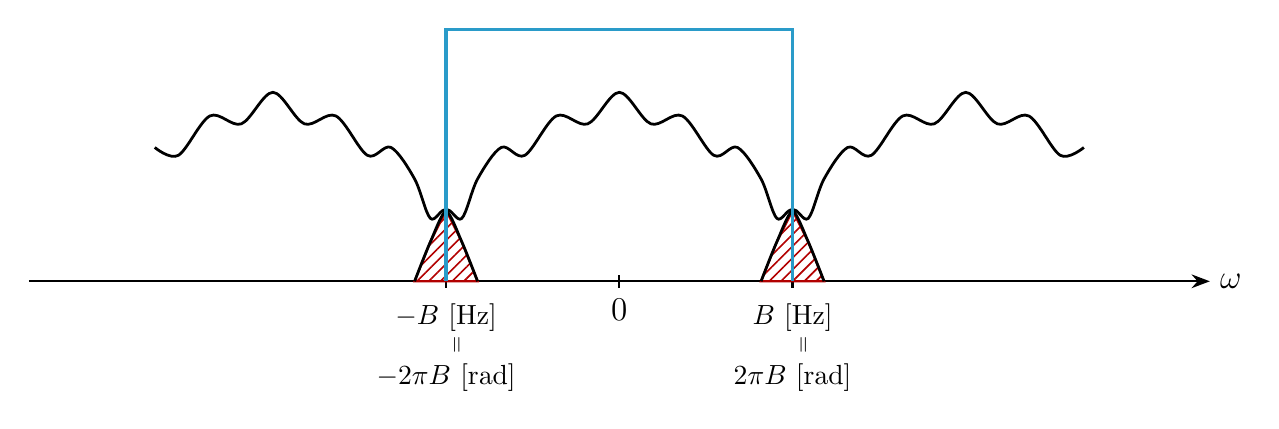
\begin{tikzpicture}[
    thick,                  % 全体の線を太めにする
    >=Stealth,              % 綺麗な矢じりを使用
    font=\large,            % フォントサイズを一括で大きくする
    % 【新設】手書き風の赤い斜線パターンのスタイル定義
    aliasing_pattern/.style={
        pattern={Lines[angle=45, distance=3pt, line width=0.6pt]},
        pattern color=red!70!black,
        draw=red!70!black,
        line width=0.8pt
    }
]

    % --- 1. 座標軸の描画 ---
    \draw [->] (-7.5, 0) -- (7.5, 0) node[right] {$\omega$};
    
    % 【原点： 0】
    \node [below=0.1cm of {0, 0}] {$0$};
    
    % 【左側：-B のラベル群】
    \node [below=0.15cm of {-2.2, 0}, font=\normalsize] (minus_B) {$-B$ [Hz]};
    \node [below=0.05cm of minus_B, font=\normalsize, scale=0.8, rotate=90] {=};
    \node [below=0.15cm of minus_B, font=\normalsize] {$-2\pi B$ [rad]};

    % 【右側：B のラベル群】
    \node [below=0.15cm of {2.2, 0}, font=\normalsize] (plus_B) {$B$ [Hz]};
    \node [below=0.05cm of plus_B, font=\normalsize, scale=0.8, rotate=90] {=};
    \node [below=0.15cm of plus_B, font=\normalsize] {$2\pi B$ [rad]};

    % 目盛りの小さな区切り線
    \draw (0, 0.08) -- (0, -0.08);
    \draw (-2.2, 0.08) -- (-2.2, -0.08);
    \draw (2.2, 0.08) -- (2.2, -0.08);


    % --- 2. 【新設】エイリアシング領域の赤斜線（ハッチング） ---
    % 波形の重なり部分の底面と交差点を結ぶパスをパターンスタイルで塗りつぶします
    % [右側の重なり]
    \path [aliasing_pattern] (1.8, 0) 
        -- (2.0, 0.5) -- (2.2, 0.9) % 右の山の左裾を登る
        -- (2.4, 0.5) -- (2.6, 0)   % 中央の山の右裾を下る
        -- cycle;

    % [左側の重なり]
    \path [aliasing_pattern] (-2.6, 0) 
        -- (-2.4, 0.5) -- (-2.2, 0.9) % 中央の山の左裾を登る
        -- (-2.0, 0.5) -- (-1.8, 0)   % 左の山の右裾を下る
        -- cycle;


    % --- 3. スペクトル波形の描画（重なり合うようにxshiftを狭めて配置） ---
    % 【中央の山】
    \draw [black, line width=1.0pt, smooth, tension=0.55] plot coordinates {
        (-2.6, 0.0) (-2.4, 0.5) (-2.2, 0.9) (-2.0, 0.8) (-1.8, 1.3) (-1.5, 1.7)
        (-1.2, 1.6) (-0.8, 2.1) (-0.4, 2.0) (0.0,  2.4) (0.4,  2.0) (0.8,  2.1)
        (1.2,  1.6) (1.5,  1.7) (1.8,  1.3) (2.0,  0.8) (2.2,  0.9) (2.4,  0.5)
        (2.6,  0.0)
    };

    % 【右側の山】（シフト幅を 5.8cm から 4.4cm に狭めてオーバーラップを発生させます）
    \begin{scope}[xshift=4.4cm]
        \draw [black, line width=1.0pt, smooth, tension=0.55] plot coordinates {
            (-2.6, 0.0) (-2.4, 0.5) (-2.2, 0.9) (-2.0, 0.8) (-1.8, 1.3) (-1.5, 1.7)
            (-1.2, 1.6) (-0.8, 2.1) (-0.4, 2.0) (0.0,  2.4) (0.4,  2.0) (0.8,  2.1)
            (1.2,  1.6) (1.5,  1.7)
        };
    \end{scope}

    % 【左側の山】（同様に左へ 4.4cm シフト）
    \begin{scope}[xshift=-4.4cm]
        \draw [black, line width=1.0pt, smooth, tension=0.55] plot coordinates {
            (-1.5,  1.7) (-1.2,  1.6) (-0.8,  2.1) (-0.4,  2.0) (0.0,  2.4)
            (0.4,  2.0) (0.8,  2.1) (1.2,  1.6) (1.5,  1.7) (1.8,  1.3)
            (2.0,  0.8) (2.2,  0.9) (2.4,  0.5) (2.6,  0.0)
        };
    \end{scope}


    % --- 4. 【新設】水色の遮断枠（理想ローパスフィルタ） ---
    % 目盛り ±B (±2.2) の位置から垂直に立ち上がるゲートを描画します
    \draw [cyan!80!black, line width=1.2pt] (-2.2, 0) -- (-2.2, 3.2) -- (2.2, 3.2) -- (2.2, 0);

\end{tikzpicture}
\end{document}

